\section{问题三：能源安全与投资—运行优化}
\subsection{可靠性约束下的投资路径}
沿用前节可比情景，安全评价采用服务交付、能源及料源约束、工程资本、重复冲击后库存恢复四个维度。年度路径要求2030—2060每年电力、各直接燃料和有用服务缺失均不超过1\%；投资决策包括三期预算、六组订单优先级及碳价漂移，共10维。每个候选从同一2024初态重新演化，投资支出通过资产建设队列，在相应投产年份转化为可用供给能力。
\begin{align}
\min_{x\in\mathcal X}\;&\big(C_{\rm cap}(x),E^{\rm net}_{2060}(x),R(x)\big),\\
C_{\rm cap}(x)&=\sum_{t=2025}^{2060}\sum_j\frac{c_{j,t}I_{j,t}(x)}{(1.04)^{t-2024}},\\
R(x)&=\max_{t\ge2030}\{r^E_t,r^D_{{\rm coal},t},r^D_{{\rm oil},t},r^D_{{\rm gas},t},r^U_t\}\le0.01.
\end{align}

\begin{figure}[H]\centering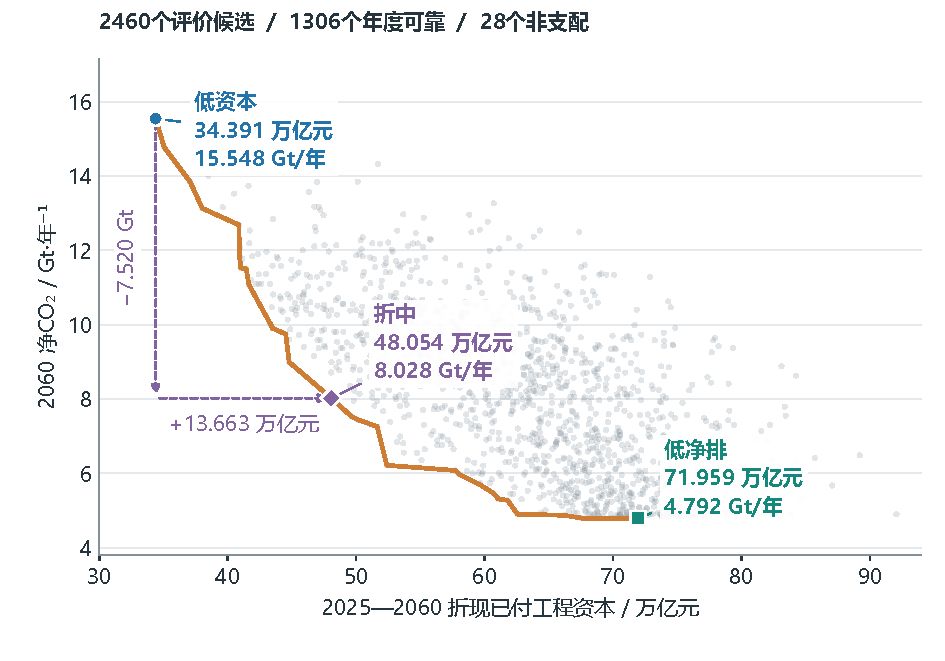
\includegraphics[width=\linewidth]{figures/figC_capital_frontier.pdf}\caption{年度可靠性约束下的资本—净排取舍。2460个评价候选中1306个年度可靠，橙线连接其中28个非支配点，三个代表点直接标注资本与净排坐标。紫色虚线箭头分解折中相对低资本的差值：资本增加13.663万亿元，2060年净排减少7.520 Gt。资本为2025—2060已付工程资本按4\%折现至2024年；技术域独立推导下界为0.175 Gt，五次固定预算搜索均未收敛。}\label{fig:figC_capital_frontier}\end{figure}

\begin{table}[H]\centering\caption{可靠性、工程资本与2060净排放的取舍}
\begin{tabular}{lrrl}\toprule
候选 & 折现资本/万亿元 & 净排/Gt & 年度可靠\\\midrule
基准参照 & 35.303 & 12.639 & 否 \\
8 Gt目标候选 & 49.643 & 7.533 & 是 \\
12 Gt目标候选 & 40.929 & 11.843 & 是 \\
最低观察净排 & 71.959 & 4.792 & 是 \\
最低观察可靠资本 & 34.391 & 15.548 & 是 \\
资本—净排折中 & 48.054 & 8.028 & 是 \\
\bottomrule\end{tabular}\end{table}

图\ref{fig:figC_capital_frontier}共评价2460个不同控制向量，1306个满足年度可靠性，形成28点已评价前沿。折中候选以48.054万亿元折现工程资本形成8.028 Gt净排路径；相对最低观察可靠资本，多投入13.663万亿元，净排减少7.520 Gt。五项固定预算搜索均达到迭代上限而未收敛，所得候选用于明确可执行的资金与技术组合。

模型2060年简化工业排放约975.346 Mt、碳汇800 Mt，能源排放非负，因而当前技术域净排下界为175.346 Mt。零净排需要扩展工业减排或新增移除能力；4 Gt目标的固定搜索尚未找到可靠候选，8和12 Gt目标已有可行路径。
\clearpage
\subsection{增量资本如何转化为不同供给组合}
折中方案多投入13.663万亿元，核水生物质、风光及燃料供应分别增加8.249、7.608、2.349万亿元，煤气发电与储能分别减少4.351、0.192万亿元。阶段长6、10、20年，年均折现增量为0.413、0.208、0.455万亿元，后期总额同时包含时间窗口长度与年均投入变化。

2060年煤气发电由14.563降至4.513 PWh，储能由179.488降至157.269 GW。三条路径均年度达标，同一连续冲击后段未供电却为0、56.870、0 TWh；这组完整组合比较说明，年度可行路径仍需冲击筛查。

\begin{figure}[H]\centering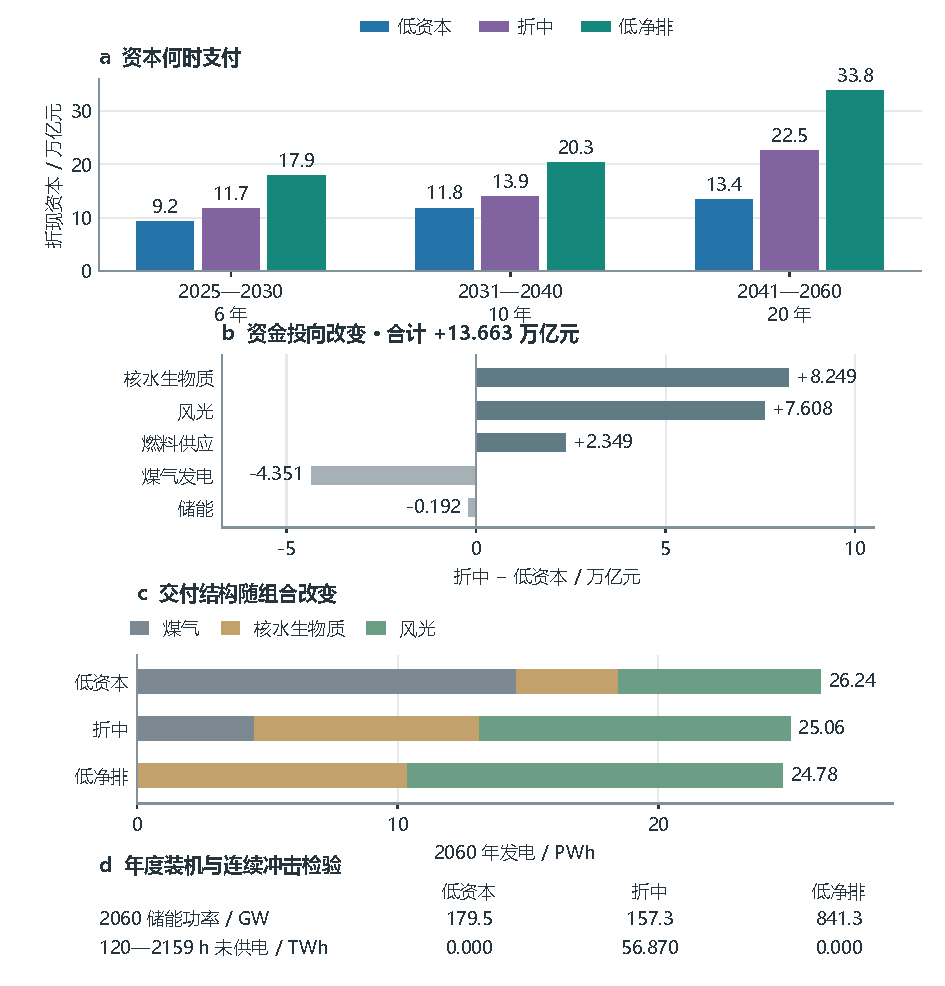
\includegraphics[width=\linewidth]{figures/figC2_investment_translation.pdf}\caption{资金投向、供给结构与冲击暴露的组合比较。a按6/10/20年分段汇总折现资本；b为折中减低资本的资金差，五组合计13.663万亿元；c为2060绝对发电量；d分列同年储能功率与连续事件h120—2159缺供。资金技术分解为完整路径的描述性分解。}\label{fig:figC2_investment_translation}\end{figure}

\clearpage
\subsection{连续小时检验与滚动协同}

\begin{figure}[H]\centering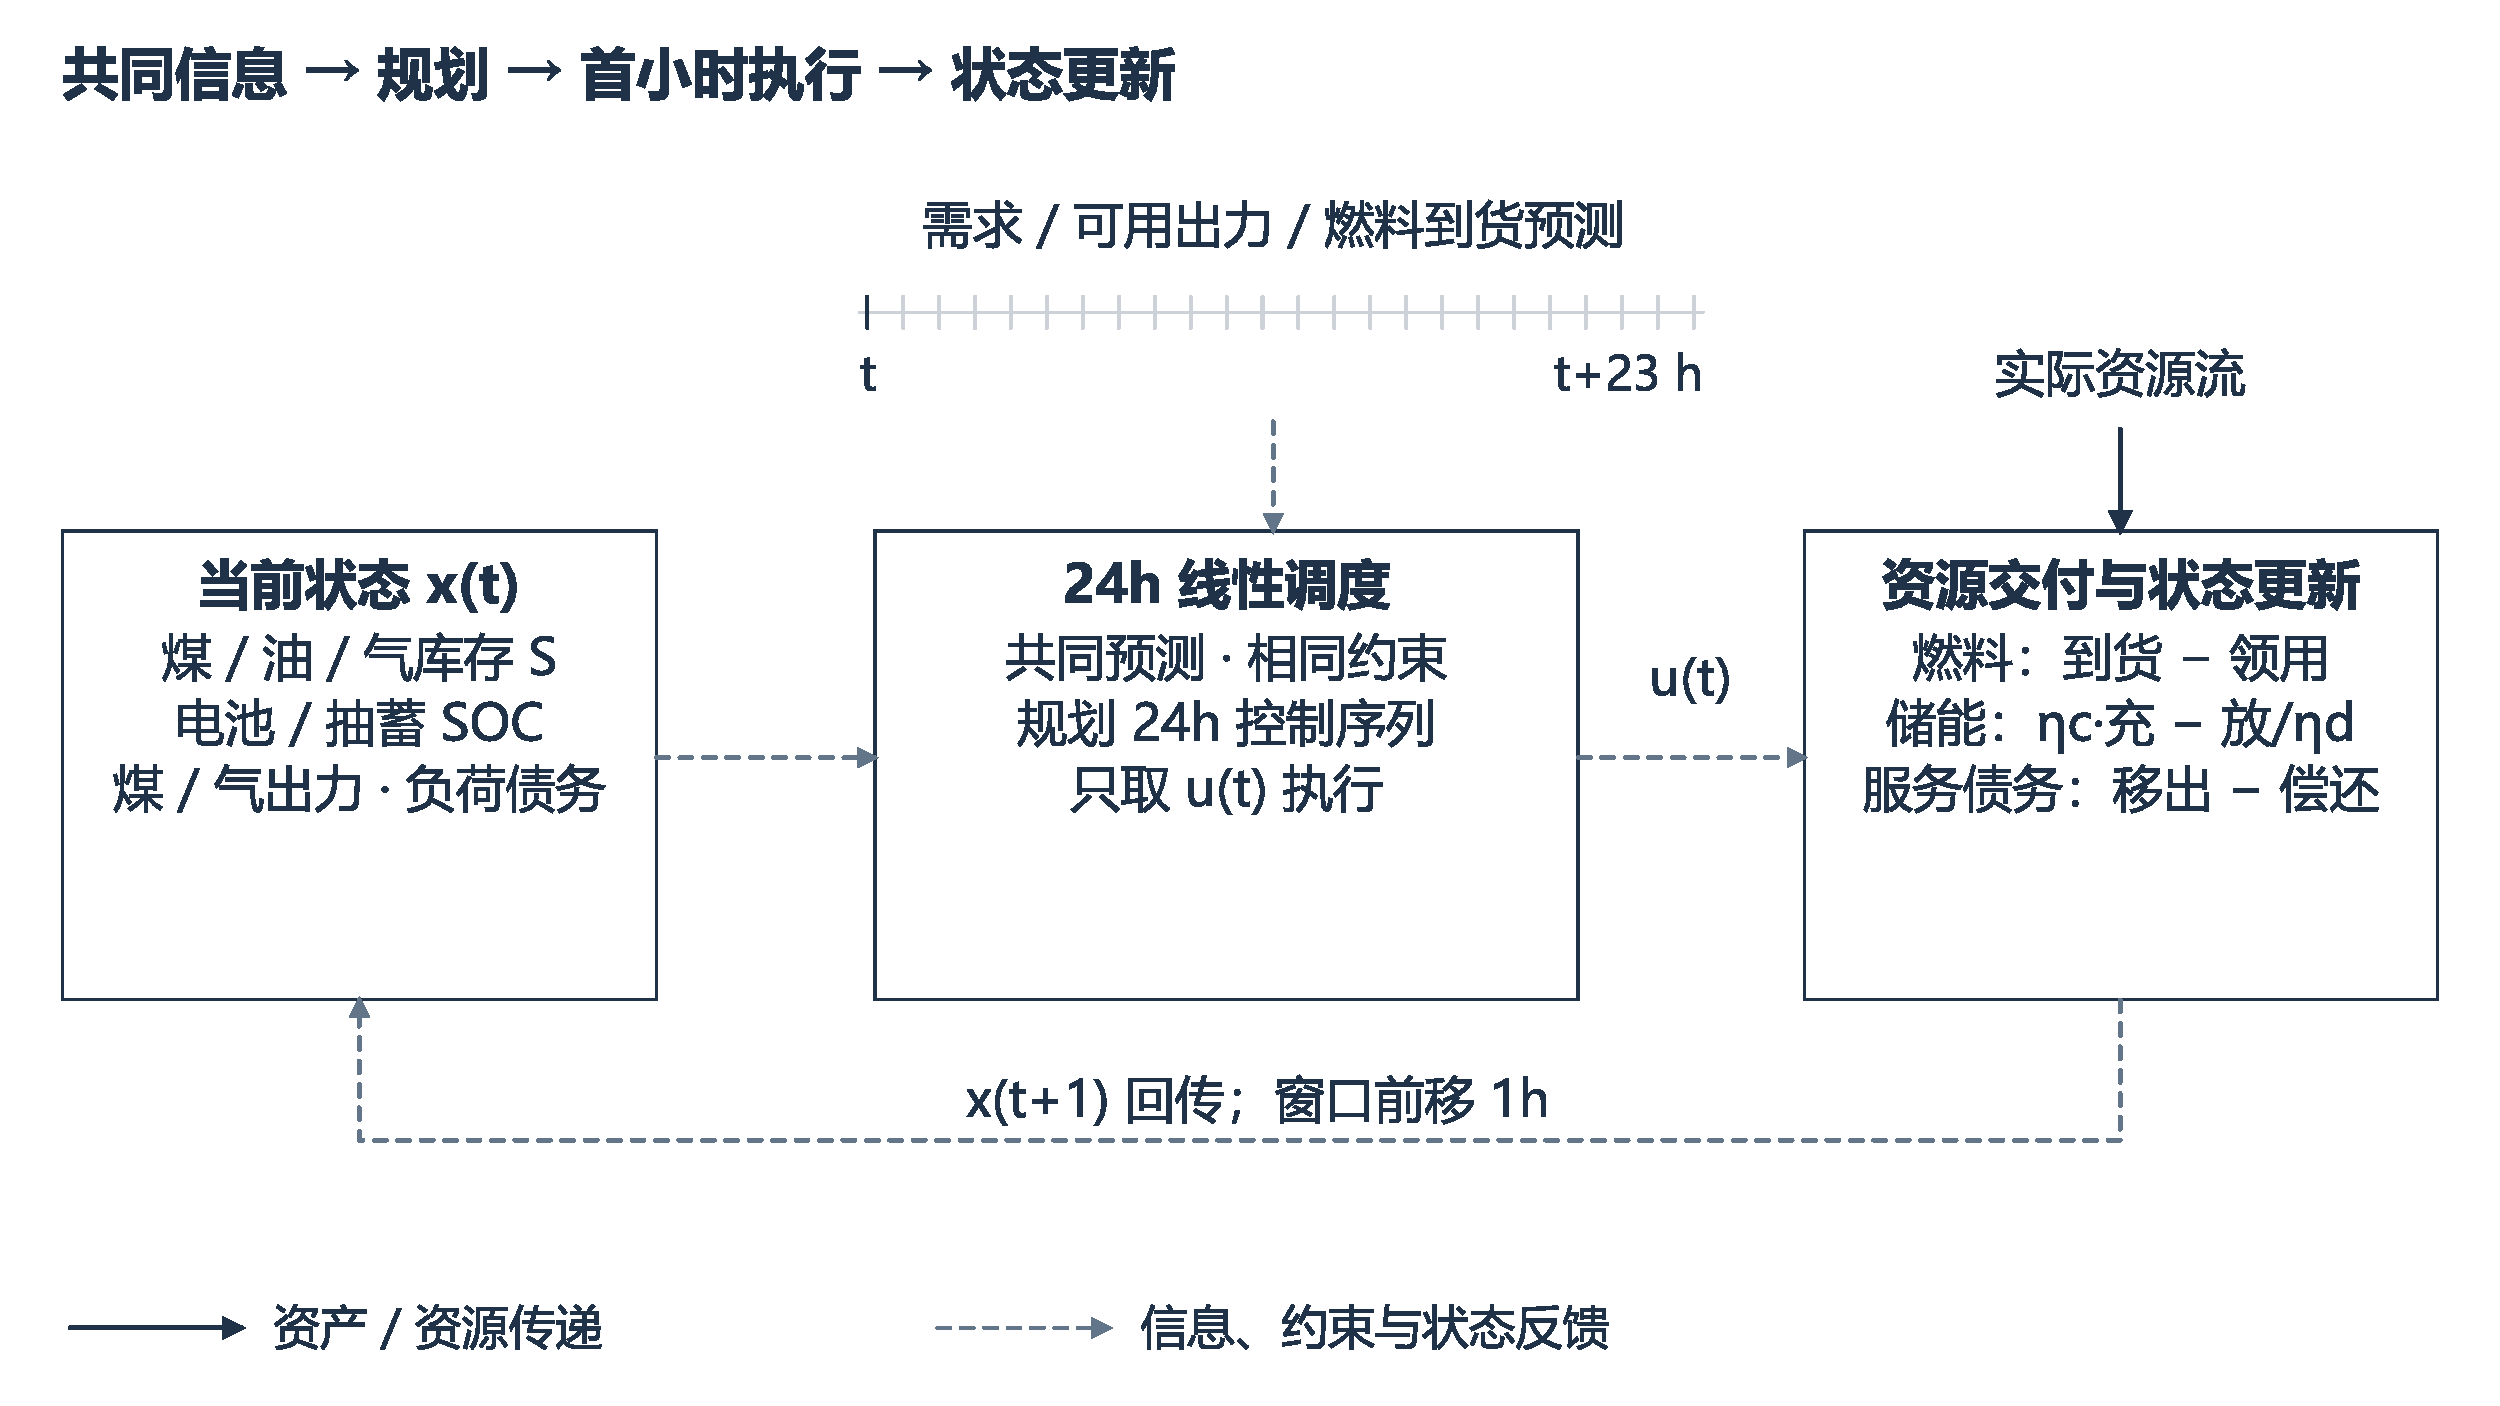
\includegraphics[width=\linewidth]{figures/fig03_rolling_control.pdf}\caption{滚动协调以当前状态和共同前瞻求解，仅执行首小时行动，再以更新库存、SOC与负荷债务进入下一小时。}\label{fig:fig03_rolling_control}\end{figure}

将三类代表投资路径的2030/2060年模拟装机、需求、料源流量、年末库存与进口渠道传入小时层。本节协调与指定非化石局部储能规则共享24小时完美前瞻，每步求解线性规划，仅执行首小时\cite{mathworks_linprog}。协调联合决定储能与资源分配；该局部规则先按需求减非化石可用出力的净负荷预期确定本地储能动作，再由同一调度器分配其余资源。燃料、SOC、热机爬坡记忆与负荷债务连续继承。
\begin{align}
S_{f,h+1}&=S_{f,h}+A_{f,h}-d_{f,h}-\mathbf1_{\{f\in\{\text{煤},\text{气}\}\}}g_{f,h}/(\eta_f\xi),\quad S_{f,h+1}\ge0,\\
E_{b,h+1}&=E_{b,h}+\eta_b^cp^c_{b,h}-p^d_{b,h}/\eta_b^d,\quad0\le E_{b,h}\le\bar E_b,\\
Z_{h+1}&=Z_h+u_h-v_h,\quad Z_{24k}=0,\quad Z_H=0,\\
g_{f,h}-g_{f,h-1}&\le R_f,\qquad0\le g_{j,h}\le\bar g_{j,h},\\
g_{f,h-1}-g_{f,h}&\le\max\{R_f,(\bar g_{f,h-1}-\bar g_{f,h})_+\},\quad f\in\{\text{煤},\text{气}\}.
\end{align}
$\xi=8141$ GWh/Mtce，煤油气化石燃烧采用IPCC默认系数\cite{ipcc}；油仅供直接服务。煤、油分别以烟煤和原油因子作聚合代表，生物源CO$_2$与生命周期排放另属其他核算范围。上爬坡受常规速率限制，下爬坡允许可用出力下降引起的受迫停机。初末库存与SOC均按同一残值计价，资源费用、合同采购现金、失供惩罚和碳价转移分别记录，生物质料源上限由年度预算传入。

每组连续运行2160小时：预运行$[0,120)$，两次冲击$[120,600)$、$[1200,1680)$，中间及末段恢复。冲击期间煤、油、气进口保留50\%、5\%、5\%，风、光、水可用出力保留25\%、55\%、70\%，电需求增加8\%。每次恢复48小时后才可有付费合同到货；合同流率不超过正常进口渠道容量50\%，每次量不超过初始库存50\%，溢价50\%。

\begin{figure}[H]\centering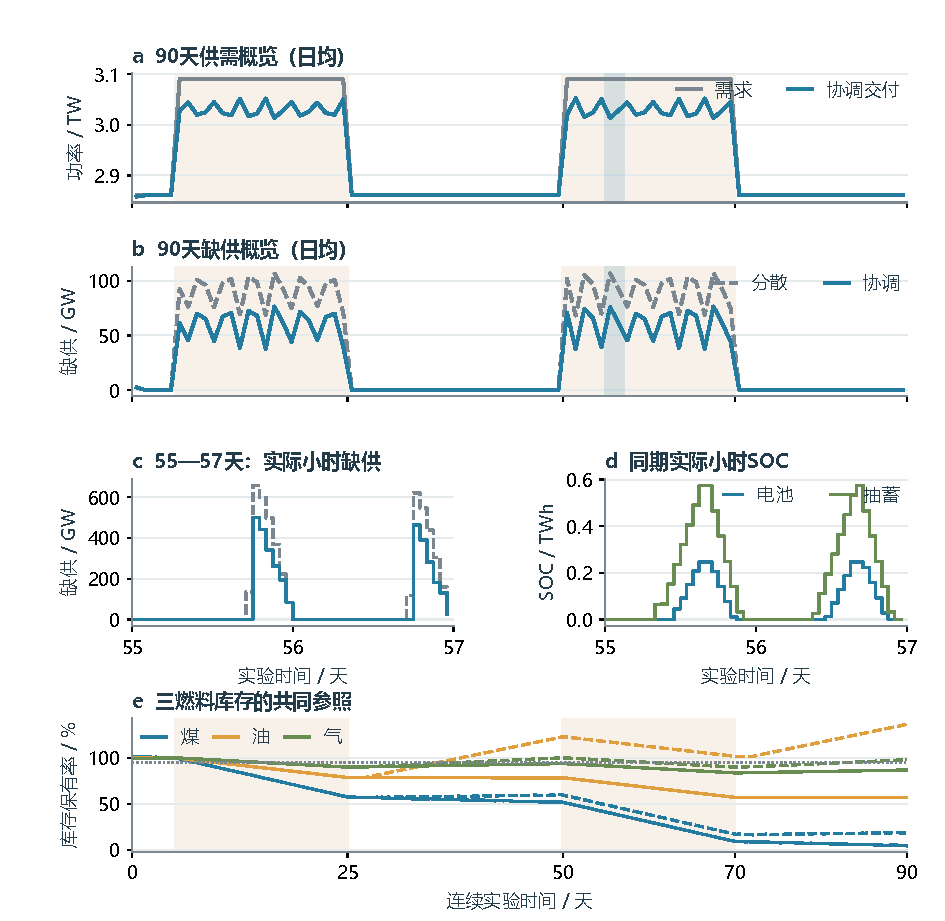
\includegraphics[width=\linewidth]{figures/figD_continuous_shocks.pdf}\caption{连续90天的运行协调与资源准备。a—b为日均功率，c—d放大55—57天实际小时缺供与SOC；浅色为两次冲击。e按三燃料各自h119库存统一归一，实线为继承供应、虚线为付费补库；95\%仅为首次事件前库存参照，不表示每次事件前归一的连续24小时联合恢复门。}\label{fig:figD_continuous_shocks}\end{figure}

\begin{table}[H]\centering\caption{继承供应下的服务交付比较}
\begin{tabular}{lrrr}\toprule
路径/年 & 预运行协调/GWh & 后续协调/TWh & 后续分散/TWh\\\midrule
最低观察可靠资本/2030 & 200.567 & 0.000 & 0.000 \\
最低观察可靠资本/2060 & 463.006 & 0.000 & 0.000 \\
资本—净排折中/2030 & 231.620 & 0.000 & 0.000 \\
资本—净排折中/2060 & 58.415 & 56.870 & 86.505 \\
最低观察净排/2030 & 109.971 & 0.000 & 0.000 \\
最低观察净排/2060 & 0.000 & 0.000 & 0.000 \\
\bottomrule\end{tabular}\end{table}

图\ref{fig:figD_continuous_shocks}中，折中2060年协调未供电为56.870 TWh，分散为86.505 TWh，减少29.635 TWh（34.3\%）；其余五类快照的预运行后电力缺失均为零。合同补库保持相同电力缺失，说明本组的新增燃料与发电可用能力约束承担不同作用。关闭煤进口渠道的同初态对照未供电上升至462.801 TWh，直接显示跨境料源对安全结果的影响。

\begin{table}[H]\centering\caption{折中2060路径的运行费用、排放与合同现金}
\begin{tabular}{lrrrr}\toprule
策略 & 后段缺供/TWh & 资源费/万亿元 & CO$_2$/Gt & 合同现金/万亿元\\\midrule
继承供应/协调 & 56.870 & 2.852 & 2.909 & 0.000 \\
继承供应/分散 & 86.505 & 2.845 & 2.894 & 0.000 \\
合同补库/协调 & 56.870 & 3.137 & 2.909 & 0.854 \\
合同补库/分散 & 86.505 & 3.130 & 2.894 & 0.854 \\
\bottomrule\end{tabular}\end{table}

费用与排放覆盖完整2160小时，缺供列为预运行后的累计值。资源费计燃料、非化石运行、储能、移峰、库存占用与合同溢价；合同全额采购现金单列。协调比同供应分散策略增加14.412 Mt排放与71.54亿元工程资源费，换取29.635 TWh交付改善。合同补库维持相同交付与排放，增加0.854万亿元采购现金并提高末期库存，反映保障储备的实际代价。
\subsection{区分服务恢复与资源恢复}
服务恢复按冲击后第一个连续24小时窗口的累计电力及各直接燃料缺供率不超过1\%判定；联合库存恢复还要求该窗口每小时三种燃料均达到各自事件前库存95\%。同一观察窗内未达到时保留未恢复状态。

\begin{figure}[H]\centering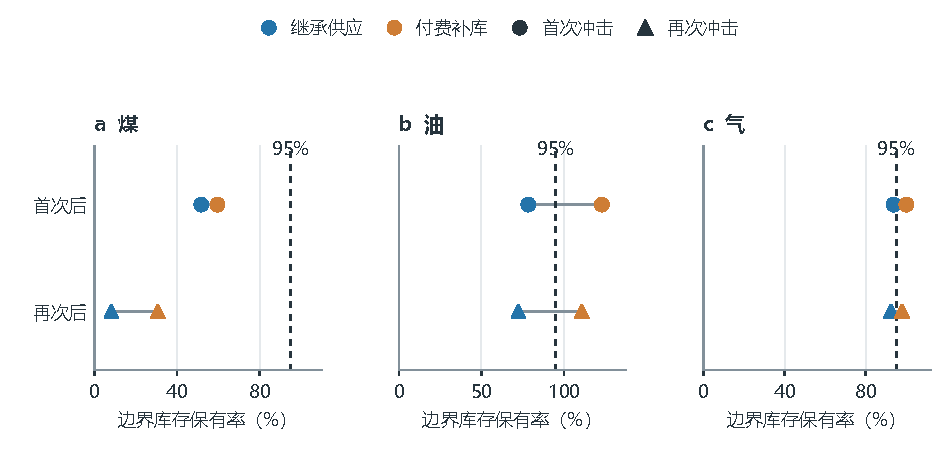
\includegraphics[width=\linewidth]{figures/fig15_service_and_stocks.pdf}\caption{服务恢复与资源准备的分离。颜色表示供给方式，形状表示冲击次数，配对线连接h1200与h2160观察边界的库存。分母为各策略各次事件前库存，95\%为对应恢复参照；与连续轨迹的首次事件前固定分母不同。}\label{fig:fig15_service_and_stocks}\end{figure}

54次事件评估中，52次首个服务窗口满足门槛，2次服务在观察窗内未恢复；全部联合库存恢复仍未达到。合同为煤提供了正到货并改善期末煤库存，三燃料的改善程度不同。零煤渠道对照则保持煤补库为零。由此，储能协调、燃料补库和建设能力应分别针对运行时序、料源和供能上限配置，服务重新达标后仍需持续追踪资源储备。

\subsection{固定投资路径的联合扰动复验}
名义可行性回答给定工程条件下能否交付，方案选择还需检验条件变化。为此固定六个既有控制，在相同48组十维开发设计中逐一评价，共288条年度路径。扰动覆盖GDP、技术成本、降本、碳价、共同资本、工期、国内供给、进口与两类行为响应；原三期控制保持不变，环境资本倍率作用于其实际预算，按2030—2060年五类服务1\%门槛比较。

\begin{table}[H]\centering\caption{六条固定路径在48组既有工程扰动中的结果}
\begin{tabular}{lrrr}\toprule
固定路径 & 年度可靠组数 & 最坏服务缺失 & 最大2060净排/Gt\\\midrule
基准参照 & 0/48 & 59.49\% & 13.432 \\
8 Gt目标 & 2/48 & 34.41\% & 10.962 \\
12 Gt目标 & 2/48 & 30.00\% & 13.948 \\
最低观察净排 & 7/48 & 34.93\% & 11.254 \\
最低观察可靠资本 & 3/48 & 35.83\% & 16.699 \\
资本—净排折中 & 3/48 & 38.74\% & 12.166 \\
\bottomrule\end{tabular}\end{table}
可靠组数直接描述这48种工程条件，最坏服务缺失取全部年份和五种服务的最大值。新增投入须与需求、料源及建设兑现共同评价；名义资本—净排前沿提供候选，扰动复验进一步识别候选需要补强的条件。每组失败的年份、载能与缺失量保留在支撑材料逐年账中。

\subsection{面向最坏服务缺失的修复及代价}
进口收缩、共同资本受限与建设延迟叠加时，直接天然气交付首先成为主要瓶颈。保供修复同时调整分期预算、燃料供给订单和发电结构，在原控制边界及资源约束内评价128组控制，每组重放48个开发条件。排序先改善最大年度载能缺失率，达到1\%后再比较名义净排与资本；固定预算搜索达到五代上限，所选方案来自预列工程组合。

\begin{table}[H]\centering\caption{固定控制的资金、净排与两类设计结果}
\begin{tabular}{lrrrrr}\toprule
控制组合 & \shortstack{折现资本\\万亿元} & \shortstack{名义净排\\Gt} & \shortstack{十维开发\\达标组数} & \shortstack{十维开发\\最坏缺失} & \shortstack{进口—工期\\达标格点}\\\midrule
原资本—净排折中 & 48.054 & 8.028 & 3/48 & 38.74\% & 5/121 \\
保供修复（方案Ⅰ） & 74.579 & 10.065 & 20/48 & 28.87\% & 52/121 \\
稳定非化石（方案Ⅱ） & 73.914 & 8.052 & 14/48 & 29.11\% & 31/121 \\
混合供给（方案Ⅲ） & 88.587 & 6.797 & 20/48 & 29.33\% & 56/121 \\
\bottomrule\end{tabular}

\smallskip\noindent 资本与净排取名义工程条件，资本按4\%折现；两类设计的达标分母分别保留。
\end{table}
\noindent{\small 方案Ⅰ、Ⅱ、Ⅲ的程序索引分别为005、006、007；编号用于检索原始控制，含义以方案名称为准。}\par

终选将三期预算倍率及统一燃料供给优先级提高到原边界上限，并提高煤电、降低气电订单优先级。开发设计内最坏服务缺失由38.74\%降至28.87\%，可靠组数由3/48提高至20/48；名义折现资本增加26.526万亿元，2060净排增加2.037 Gt。非化石与混合组合展示了不同减排代价，表中仍按原排序保留终选。

终选方案在另48组独立联合设计中21组满足年度门槛，最坏缺失30.51\%，出现在2030年直接油服务。该设计把油供应工期由3年延长至6年，2025年新订单到2031年才投产；2030年油请求1117.490 Mtce、交付776.595 Mtce、库存为零，而资本支出2.865万亿元低于6.255万亿元预算。即时约束已由资金转为建设兑现：追加当期预算不能使既定工期的订单提前供能，应优先核对截止前可投产队列与外部料源。开发选择与独立检验的分离见统一验证说明。

\subsection{进口与建设工期下的已检验适用条件}
为分离料源与建设兑现，固定四个既有控制，在进口可用倍率0.50—1.10与新订单工期倍率1.00—2.00的11$\times$11网格上比较，共484条年度路径，名义点另列。进口倍率持续作用于可用渠道，工期倍率作用于新订单及原有预期规则，初始在建队列保持原值；每点均要求2030—2060年逐年五类服务缺失不超过1\%。

\begin{figure}[H]\centering
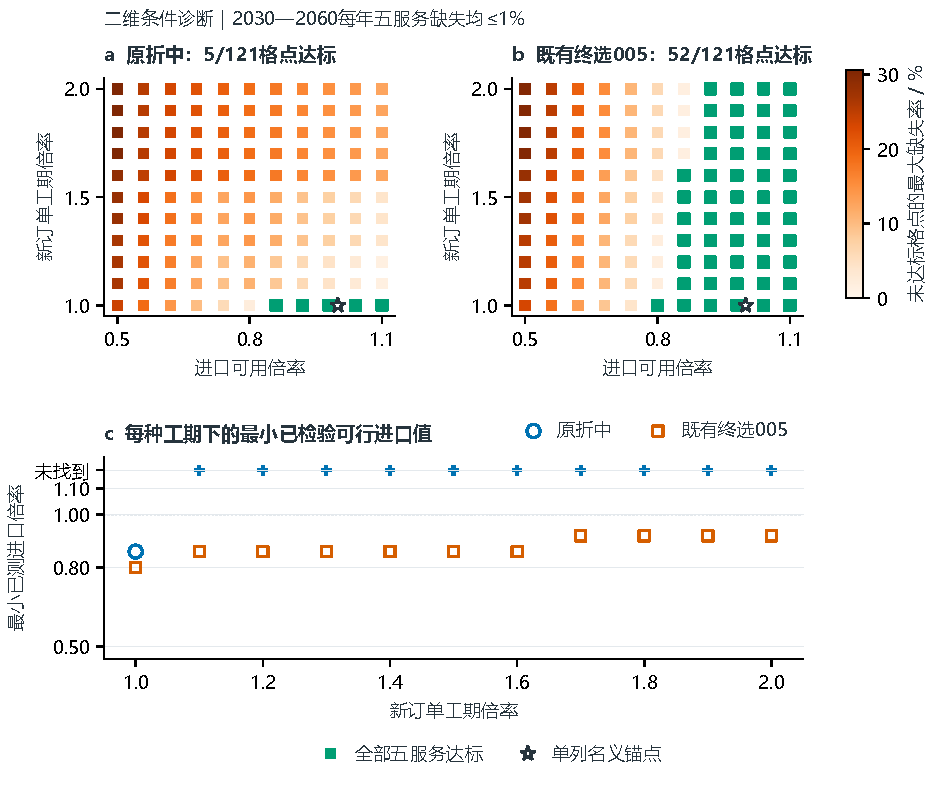
\includegraphics[width=160mm]{figures/figK_fixed_control_safety_envelope.pdf}
\caption{固定控制的进口—工期安全域。格点为实际测试组合，绿色满足2030—2060逐年五服务缺供$\le$1\%，橙色为最大缺失率；星号是单列名义锚点。下图仅连接每种工期最小的已测可行进口倍率，含工期1名义点；叉号表示已测试进口值中未找到可行点。}
\label{fig:fixed-control-envelope}\end{figure}

原折中在121点中仅5点达标，均为工期倍率1.00、进口倍率至少0.86的已测组合。保供修复（方案Ⅰ）增至52点：工期1.00的最小已测可行进口倍率为0.80，工期1.10—1.60为0.86，工期1.70—2.00为0.92。稳定非化石（方案Ⅱ）与方案Ⅲ分别为31、56点，形成不同资本与净排取舍。这里的点数衡量相同网格中的覆盖，图中标记用于选择已检验条件；两轴以外的条件仍由十维联合设计另行评价。

这一台阶直接对应油项目投产时点。对方案Ⅰ固定进口0.86，工期倍率从1.60增至1.70时，油新订单工期由5年取整为6年，2025年订单从2030年投产变为2031年投产；截至2030年，新订单形成的油能力由16.016降为0 Mtce/年，初始队列投产保持23.877 Mtce/年。2030年同为1195.631 Mtce的油请求，交付由1190.307降至1178.434 Mtce，缺失率由0.445\%升至1.438\%。保持工期1.70、将进口提高至已测0.92，油缺失归零且全部年份五服务达标，形成“投产台阶—油服务缺口—进口条件”的逐项见证。

进口增加不能代替全部建设。进口倍率1.10、工期2.00时，四个控制的2030年直接油服务均满足需求，但原折中仍在2031年出现12.44\%直接气缺失，稳定非化石（方案Ⅱ）仍在2030年出现2.72\%电力缺失。补充跨境料源可解除油供给约束，直接气与发电竞争、供给和电源建设兑现仍须共同检查。因此，早期油气交付先用渠道与订单时点核算，再按实际载能缺口配置电源；工程方案的适用条件应与资本和减排代价同时呈现。
进口倍率在本图中表示供给条件，表中资本为实际工程投资；保障额外进口能力的费用需另行核算。


\subsection{油气订单的有效建设窗口与2030年交付}
进口—工期网格揭示了投产台阶。进一步固定原保供修复方案及48组开发设计和名义条件，比较四种建设机制：P0为原提案与同比例支付；P1在油气不晚于2030年投产时优先付款；P2在有效窗口补至原物理建设上限并优先付款；P3全期均补至上限并优先付款。四臂共196条2025—2060年完整路径，在相同逐年预算金额下识别建设时点与组合结构的作用。

有效窗口由已知工期决定：$E_{f,t}=\mathbf{1}\{t+\lceil L_f d\rceil\leq2030\}$。油工期4、5、6年时，最后有效订单年分别为2026、2025、2024；气工期3、4年时分别为2027、2026。年建设上限、初始队列、退役、当期预算公式和进口演化沿用基准模型参数与演化方程。优先组资金不足时在组内按比例支付，剩余资金再分配给其他提案。本次四臂逐案逐年的实际预算金额相同，折现实付资本按实际订单另行累计。
\begin{table}[H]\centering\caption{建设时点机制的完整开发组与名义情景结果}
\begin{tabular}{lrrr}\toprule
机制 & 全年度可靠 & \shortstack{名义折现资本\\万亿元} & \shortstack{名义2060净排\\Gt}\\\midrule
原方案Ⅰ & 20/48 & 74.579 & 10.065 \\
有效窗口优先支付 & 20/48 & 74.579 & 10.065 \\
有效窗口补建设上限 & 20/48 & 74.936 & 10.076 \\
全期补建设上限 & 19/48 & 76.906 & 13.869 \\
\bottomrule\end{tabular}
\smallskip\par\noindent 可靠要求2030—2060各年电力、三种直接燃料及有效服务缺失均不超过1\%；48组为固定工程设计。
\end{table}
窗口优先支付在第38、39号设计增加气订单，第38号2030年气缺口降低0.419个百分点，但油缺口仍约24.396\%。窗口扩建P2在6组设计降低当年油缺口，完整年度可靠数仍为20/48；第32号原已达标，另五组仍未越过1\%门槛。全期扩建P3则降至19/48：高增长、低预算与进口收缩的第21号设计在2060年新增1.025\%电力缺失，折现资本由69.737增至71.075万亿元、净排由11.447增至14.471 Gt，以上差值均以原机制P0为参照。

第21号设计的全期油气扩建改变了共同资本配置和后续主体反馈。相对P0，2060年风光发电减少3158.661 TWh、煤电增加3687.398 TWh，总发电仍减少238.841 TWh；同时需求增加59.611 TWh，合成298.452 TWh电力缺口。局部燃料能力增长因此没有转化为全期可靠改善，应沿完整资产组合、实际投产和需求响应共同评价。

这一组负结果把措施落实到投产时钟：油工期6年时，2025年后的新订单均晚于2030；当期优先付款改变资金分配，却不改变既定工程周期。对具体年份的缺口，先核对已有队列、可在截止前形成的国内供给、进口和可释放库存，再确定建设与外部资源保障的组合。
\begin{figure}[H]\centering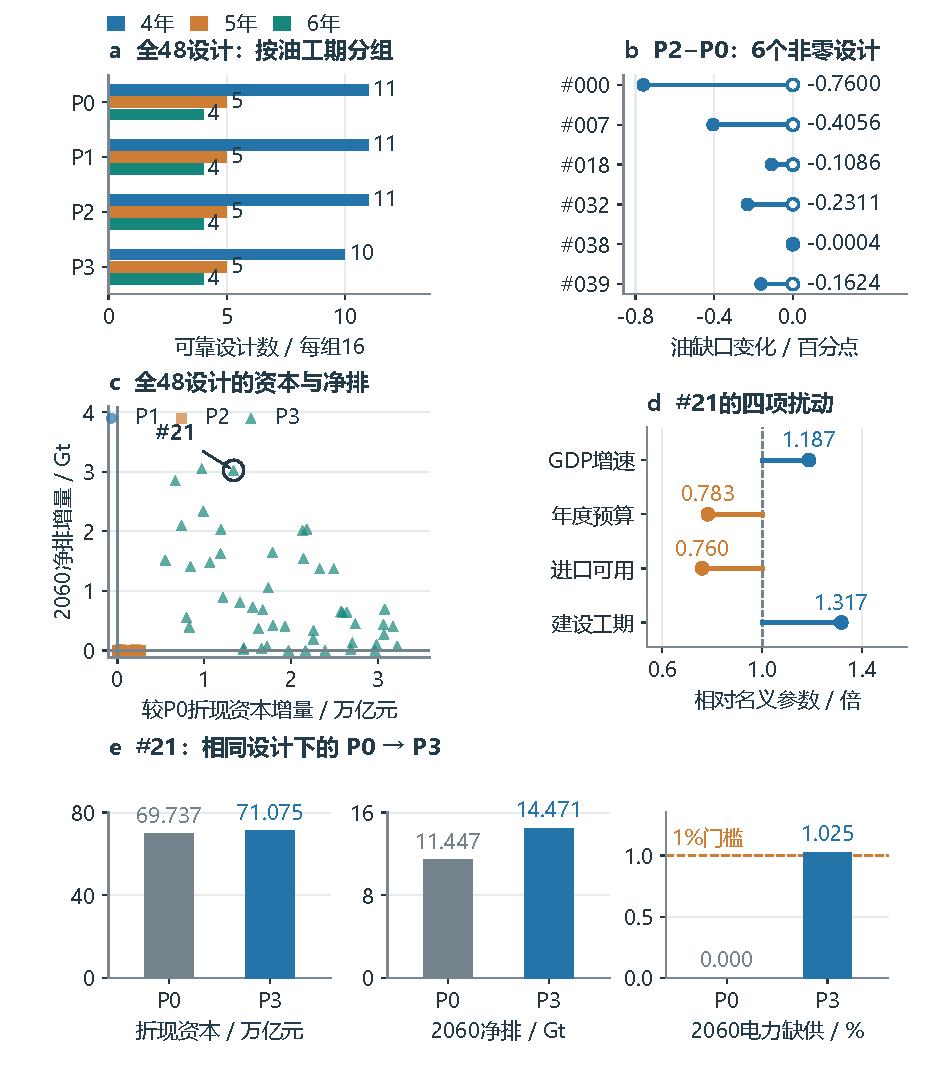
\includegraphics[width=\linewidth]{figures/figP_deadline_investment_mechanisms.pdf}\caption{建设时点机制的完整开发域比较。a按油工期分组，每组16个设计；全48设计可靠数为20/20/20/19。b显示P2相对P0油缺口的6个非零差，其余42组该指标为数值零。c保留全部48设计的资本—净排变化。d以名义值1标记第21号设计的四项扰动；e分别以完整坐标比较该设计P0与P3的资本、净排及电力缺供，1\%虚线为可靠门槛。资本按4\%、2024原点折现；净排和电力缺供取2060年度。}\end{figure}

\subsection{把年度投资组合落实到小时交付}
新增投资—运行、库存参照及运行条件试验统一采用SciPy/HiGHS逐时重优化，逐步反馈实际状态；原生实现证据在下一节单列。各轮协议和源程序在求解前固定，保存全部输入与逐时动作。

固定原折中、方案Ⅰ、方案Ⅱ和方案Ⅲ四个控制，将各自2030、2060年需求、装机、实际国内与进口料源流量和年末燃料库存传入同一360小时设计；每个快照各执行协调与原非化石局部储能规则，共16条完整路径、5760小时。方案Ⅰ使用实际年度原生复验输出，方案Ⅱ与方案Ⅲ由冻结控制重建年度轨迹；原折中2060的两条路径先逐列复现既有试验。各快照以50\%储能SOC、零热机记忆和零移峰债务初始化，之后连续反馈自身状态。该试验比较年度资产在相同工程事件中的交付，年度库存沿用各自轨迹，储能SOC采用统一设计初态。

\begin{figure}[H]\centering
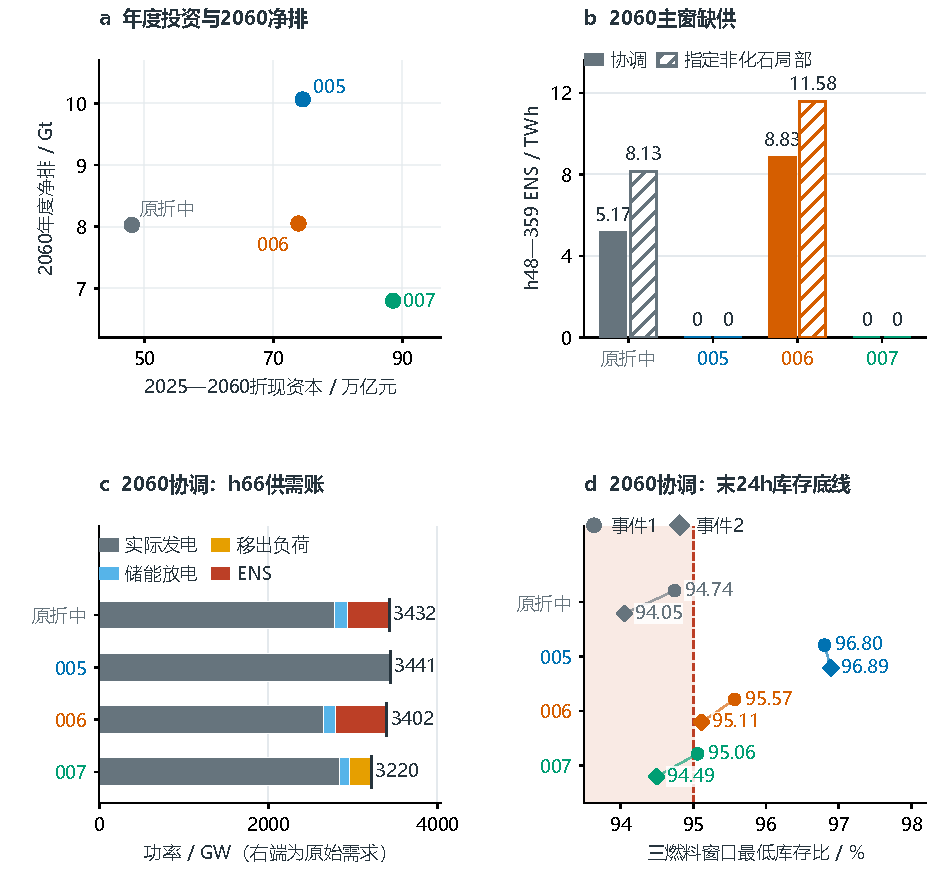
\includegraphics[width=160mm]{figures/figL_annual_operations_choice.pdf}
\caption{年度组合在小时层的实际交付。a为2025—2060折现资本与2060净排，b为h48—359缺供，c在共同h66核对供需；d为两次边界前24小时三燃料最低库存比，分母为各方案各事件前库存。2030八条路径主窗缺供均数值为零（绝对值$\le$$10^{-8}$GWh），完整360小时含预运行。}
\label{fig:annual-operations}\end{figure}
\begin{table}[H]\centering\caption{四个投资组合的协调运行：主评价窗与完整路径}
\begin{tabular}{lrrrrr}\toprule
组合 & \shortstack{2030主窗\\TWh} & \shortstack{2030全段\\GWh} & \shortstack{2060主窗\\TWh} & \shortstack{2060全段\\TWh} & \shortstack{2060主窗峰\\GW}\\\midrule
原折中 & 0.000 & 231.620 & 5.170 & 5.228 & 494.114 \\
方案Ⅰ & 0.000 & 224.241 & 0.000 & 0.188 & 0.000 \\
方案Ⅱ & 0.000 & 249.313 & 8.827 & 8.941 & 604.636 \\
方案Ⅲ & 0.000 & 96.235 & 0.000 & 0.000 & 0.000 \\
\bottomrule\end{tabular}
\smallskip\par\noindent 主窗为第48—359小时，全段为第0—359小时；小于$10^{-6}$ GWh的缺供按数值零展示，原始浮点值保留。
\end{table}

2060年方案Ⅰ与方案Ⅲ在主窗的电力缺供为数值零，方案Ⅱ为8.827 TWh，高于原折中的5.170 TWh。方案Ⅰ全360小时仍有187.839 GWh初始化缺供，四个2030快照的缺供也集中在初始化。年度服务达标与冲击交付因而须分别检验。

共同第66小时给出了组合差异的物理见证。方案Ⅰ需求3440.920 GW由实际发电完全覆盖，煤电出力2504.227 GW，距可用上限仍有244.887 GW。方案Ⅱ需求3401.528 GW虽低于原折中30.636 GW，发电可用上限却减少126.726 GW、储能交付功率减少14.432 GW；七类电源均达到当期上限，两储能仍有能量而触及放电功率上限，最终缺供604.636 GW，比原折中高110.521 GW。方案Ⅲ则以2844.383 GW发电、118.250 GW放电和257.620 GW负荷移出满足3220.253 GW需求。这些守恒账将资本转换为整套供给结构和时序动作，支持按实际缺口配置资产。

表中年度剩余净排以Gt计；小时燃烧CO$_2$与资源费用另行累计。2060协调完整360小时，原折中、方案Ⅰ、方案Ⅱ、方案Ⅲ的燃烧CO$_2$分别为439.721、473.313、428.412、390.363 Mt，资源费用分别为454.819、472.326、450.234、449.337十亿元。资源费含到货与净库存/SOC领用计价、运行和库存占用，不含缺供惩罚、碳价转移及新增工程资本。

\subsection{库存恢复采用三种参照回答三个问题}
方案Ⅰ在原事件前库存参照下，两次末24小时煤库存底线为96.80\%、96.89\%，两次服务与联合库存窗口均达标且随后保持；方案Ⅲ第二次底线为94.49\%，在第290小时再跌破。为进一步分离累积领用和事件增量，对上述16条冲击路径各增算一条同初态、同需求日型、同控制的无事件路径，共5760小时。新增路径只去除事件对可用出力、需求和进口的扰动。

定义$A_e=\min_{h\in W_e}S_h/S_{e,\rm pre}$，衡量相对最近事件前的恢复；$B_e=\min_{h\in W_e}S_h/S_0$，衡量相对试验初始储备的保持；$C_e=\min_{h\in W_e}(S_h/S_h^{\rm normal})$，衡量同小时无事件路径的资源差距。$W_e$取对应观察边界前24小时，$C_e$按逐小时比值取最小。原95\%恢复判定继续使用$A_e$，新增$B_e,C_e$用于解释库存演化。
\begin{table}[H]\centering\caption{2060协调路径第二次末24小时的煤库存及期末事件增量}
\begin{tabular}{lrrrr}\toprule
组合 & $A_2$/\% & $B_2$/\% & $C_2$/\% & \shortstack{期末额外领用\\Mtce}\\\midrule
原折中 & 94.05 & 88.95 & 91.95 & 30.461 \\
方案Ⅰ & 96.89 & 94.76 & 91.49 & 34.545 \\
方案Ⅱ & 95.11 & 90.93 & 92.14 & 30.303 \\
方案Ⅲ & 94.49 & 89.72 & 92.08 & 30.160 \\
\bottomrule\end{tabular}
\smallskip\par\noindent 额外领用为无事件期末库存减冲击期末库存；三列比例分别采用事件前、固定初始和同小时无事件库存作为分母。
\end{table}

方案Ⅰ相对最近事件前已恢复，但相对固定初始库存的第二次窗口底线为94.76\%，相对同小时无事件库存为91.49\%。其期末煤库存为372.181 Mtce；无事件路径本会累积至406.726 Mtce，两者相差34.545 Mtce。原折中相应事件增量为30.461 Mtce。三种参照共同表明：方案Ⅰ改善了供给组合与相对事件前的准备，持续资源保障还须计入正常演化的库存目标。原库存费用已包含资源净领用，表中额外领用按实物量报告。

\subsection{补库购买了哪些准备：现金、资源与目标分账}
在四个2060资产组合上各比较继承原到货与原付费应急合同，共8条360小时完整路径。合同按预定事件日历，在事件结束12小时后追加进口；总流量最高为原年进口能力折小时的150\%，因而需要额外通道余量。三燃料新增到货分别为煤10.623、油23.553、气6.046 Mtce；每条路径的非库存动作、缺供、峰值与CO$_2$均与对应原到货路径相同，增量到货全部留为期末库存。

每方案新增采购现金为1666.523亿元，其中基价1111.016亿元形成新增期末燃料资产，溢价555.508亿元构成物理资源净增费。沿用同一工程单位价值，采购现金与资产形成分别列账；运输扩容资本和融资费用另需工程项目数据。

以最近事件前库存为参照A，原折中与方案Ⅲ的第二次窗口由未持续达标转为达标，首次联合确认时刻仍为119、263小时。以固定初始库存为参照B，合同后的四方案第二次窗口最低比率依次为91.601\%、97.223\%、93.526\%、92.306\%；以原继承到货、无事件资源路径为参照C，依次为94.440\%、93.800\%、94.583\%、94.553\%。A回答相对最近事件前的恢复，B回答期初资源保持，C回答原无事件资源目标下的准备程度。该合同增购准备，原资源目标仍给出后续补充量。
\begin{figure}[H]\centering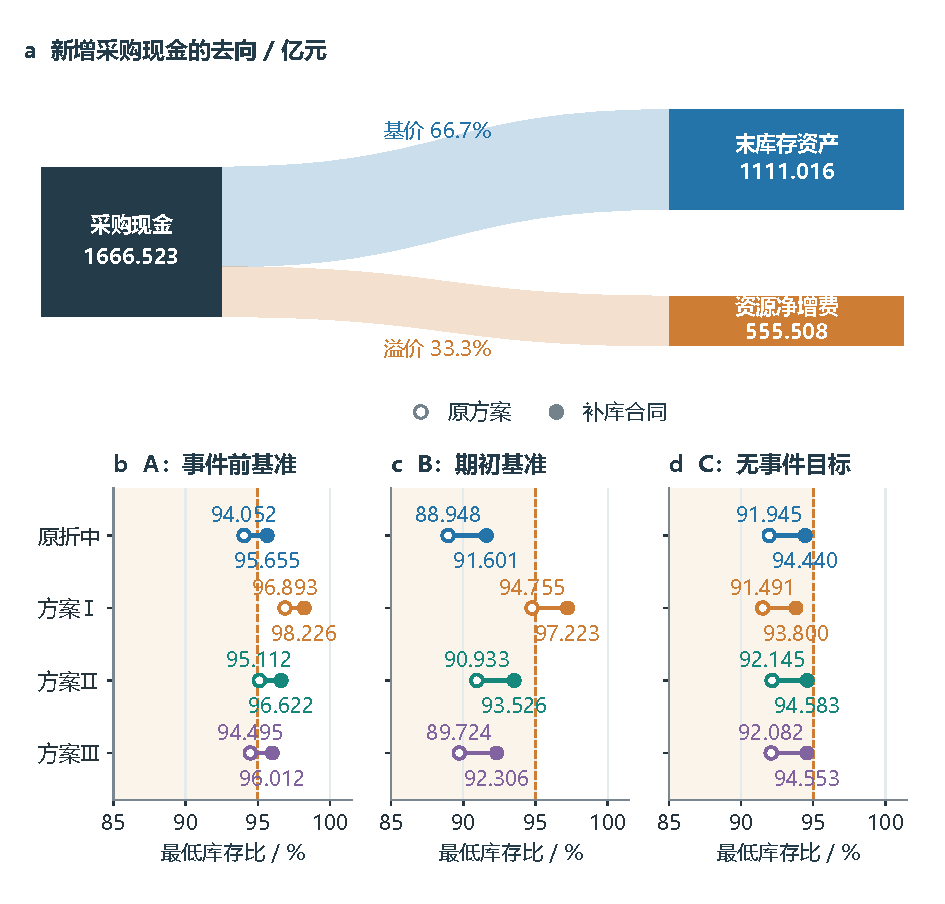
\includegraphics[width=\linewidth]{figures/figN_replenishment_cash_and_readiness.pdf}\caption{补库的现金分解与资源准备。a按实际金额比例将1666.523亿元采购现金分为1111.016亿元新增末库存资产和555.508亿元溢价，后者等于物理资源净增费；基价不重复计入资源净耗费。b—d显示h336—359逐燃料、逐小时库存比最低值，空心原方案→实心合同。A、B、C分别以自身事件前库存、自身期初库存及相同资产下原无事件资源路径为参照；95\%虚线为相应参照值。}\end{figure}

\FloatBarrier
